\chapter{Développements Logiciel : Conception, Modélisation, Implémentation} 

\section{Développements logiciel}
Dans le cadre du projet, plusieurs éléments ont été développé, à noter, une intelligence artificielle pour détecter des seiches dans une image, une base de donnée de seiche pour entrainer l'intelligence artificielle et un algorithme de filtre à particule utilisant des descripteurs et mesures de similarité pour calculer le poids de chaque particules.\\

\subsection{Intelligence Artificielle}
La base de donnée d'image de seiche est composé d'image provenant de vidéos de seiche prisent par des plongeurs en mer, et par des particuliers dans des aquariums.\\
Chaque image a été annotée à la main par les membres du groupe en utilisant le logiciel en ligne Roboflow, la base de donnée est constitué d'un total de 5175 images.\\
L'intelligence artificielle utilise le code et les poids pré entrainé de YOLOv7\cite{wang_yolov7_nodate}, qui peuvent être trouver sur le github officiel de YOLOv7\cite{yolov7_github}.
Cette intelligence artificielle a été entrainé pour 300 cycles de la base de donnée, soit un total de 25 heures sans interruptions.\\
Les performances obtenues sont illustrées dans la figure \ref{fig:ai_results} et des exemples sont donnés en figure \ref{fig:ai_examples}.\\

\begin{figure}[!htbp]
\center
	\subfloat[Precision]{{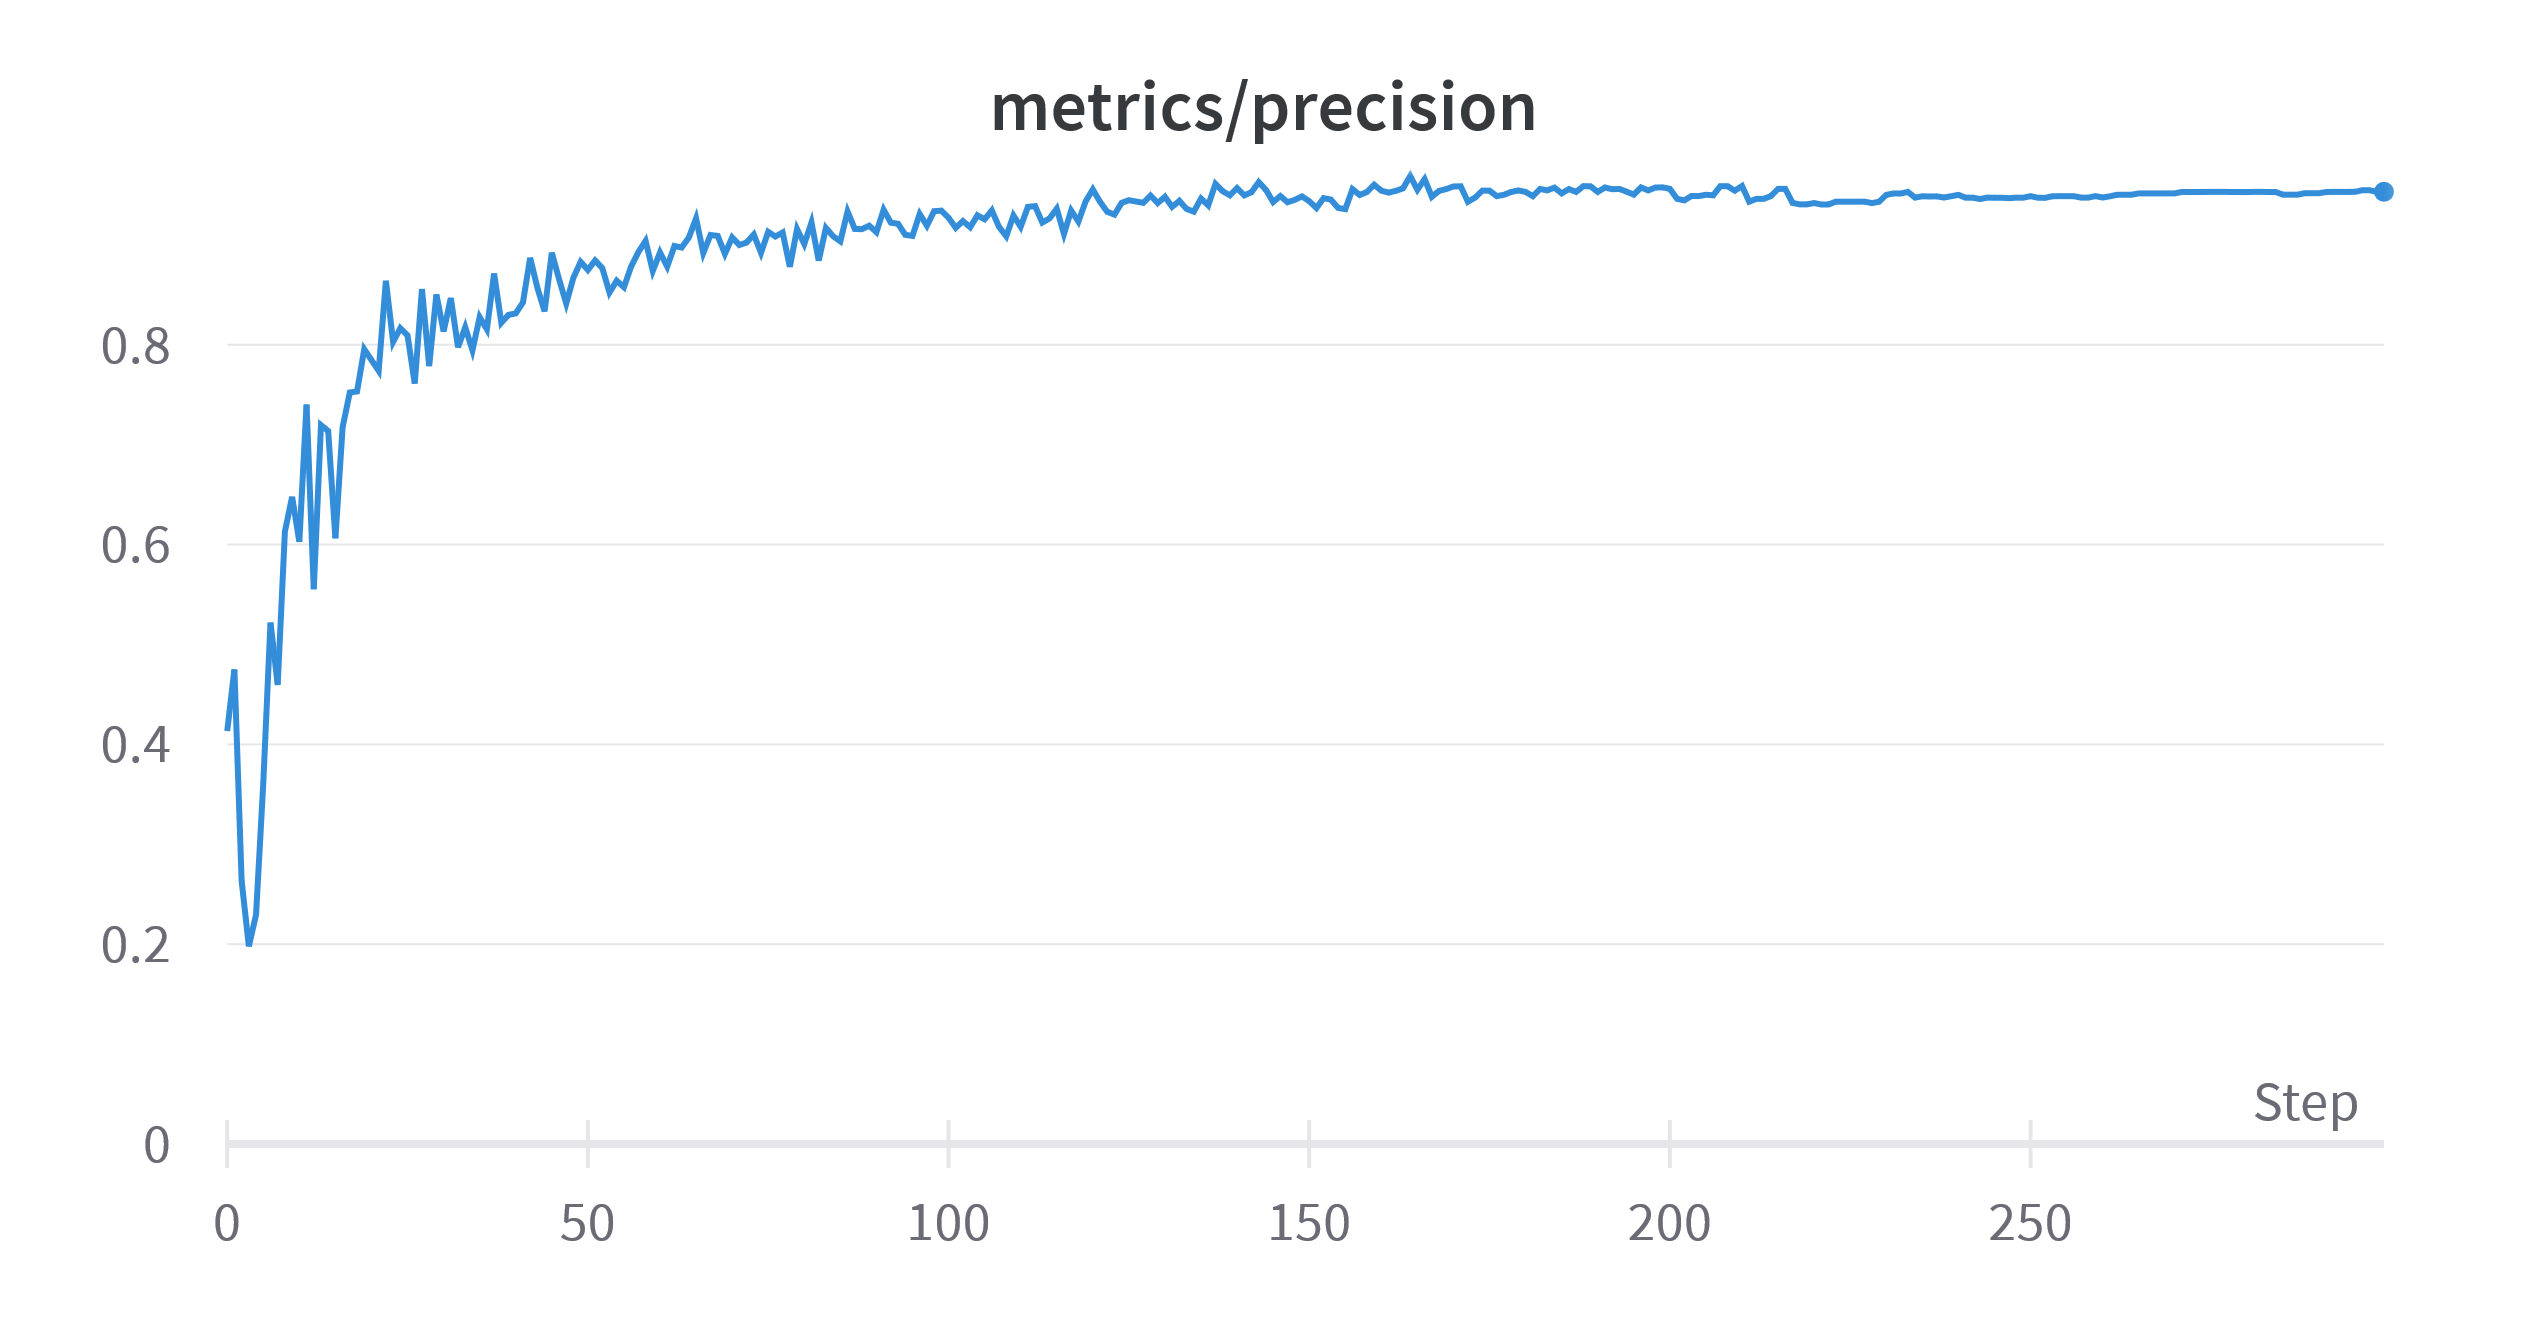
\includegraphics[scale=0.07]{metricsprecision.png}}}
	\subfloat[Recall]{{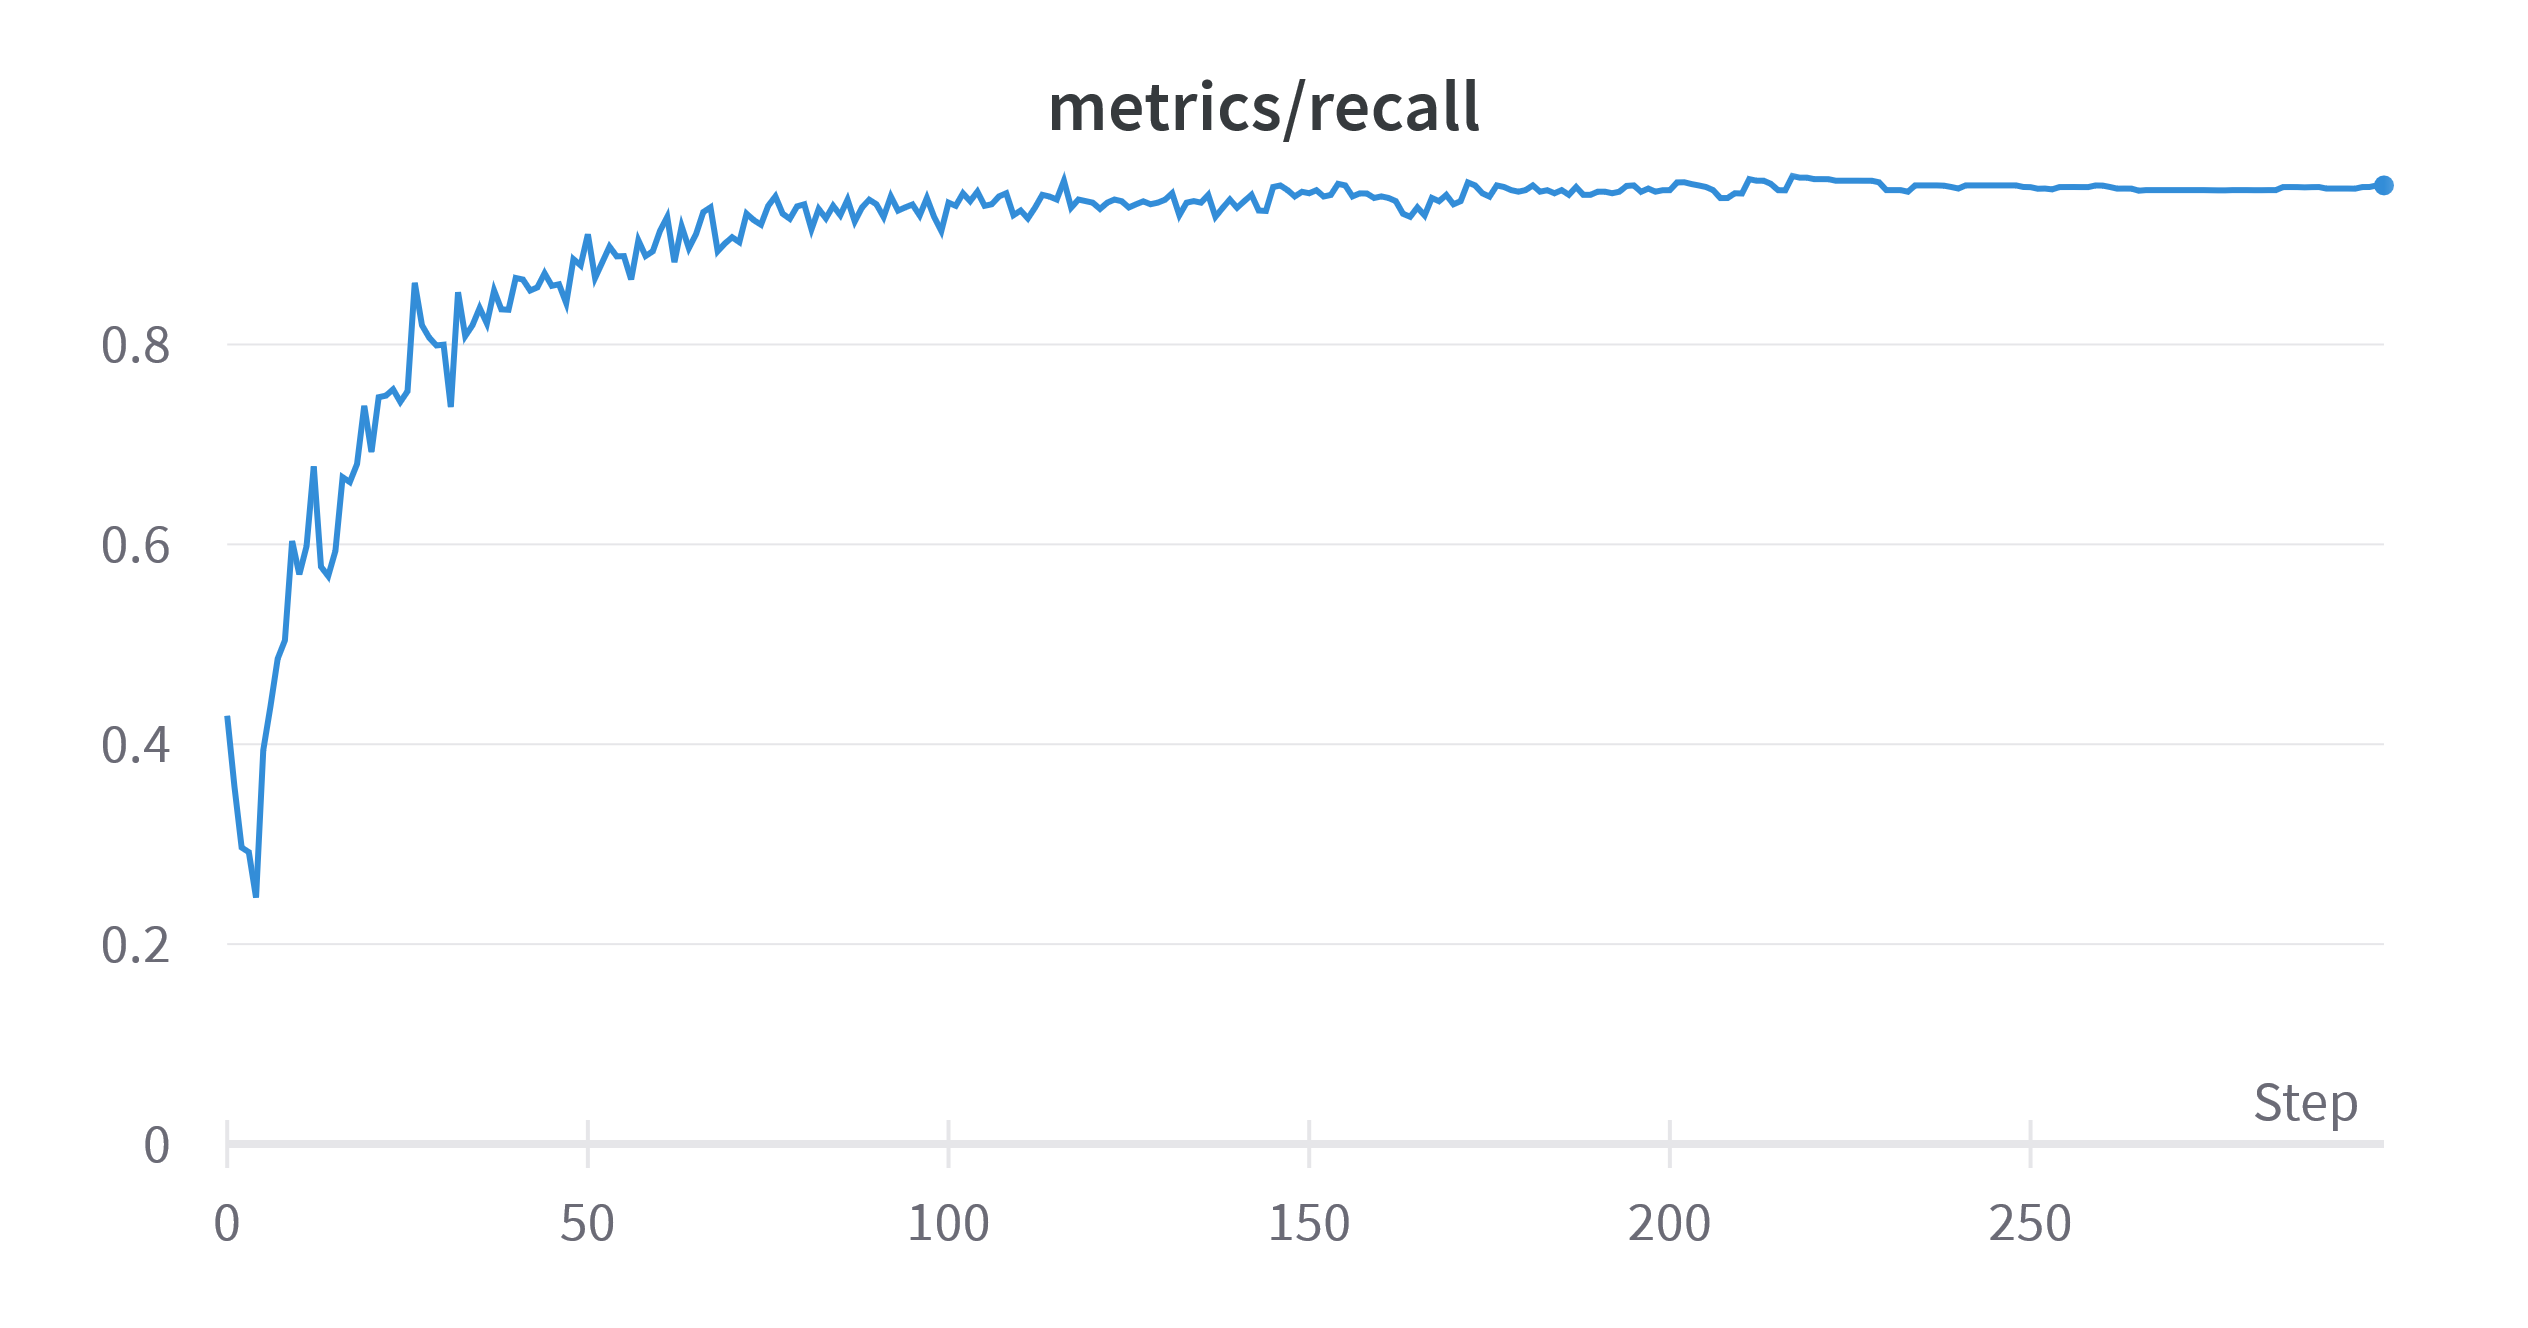
\includegraphics[scale=0.07]{metricsrecall.png}}}
	\\
	\subfloat[mAP@.5]{{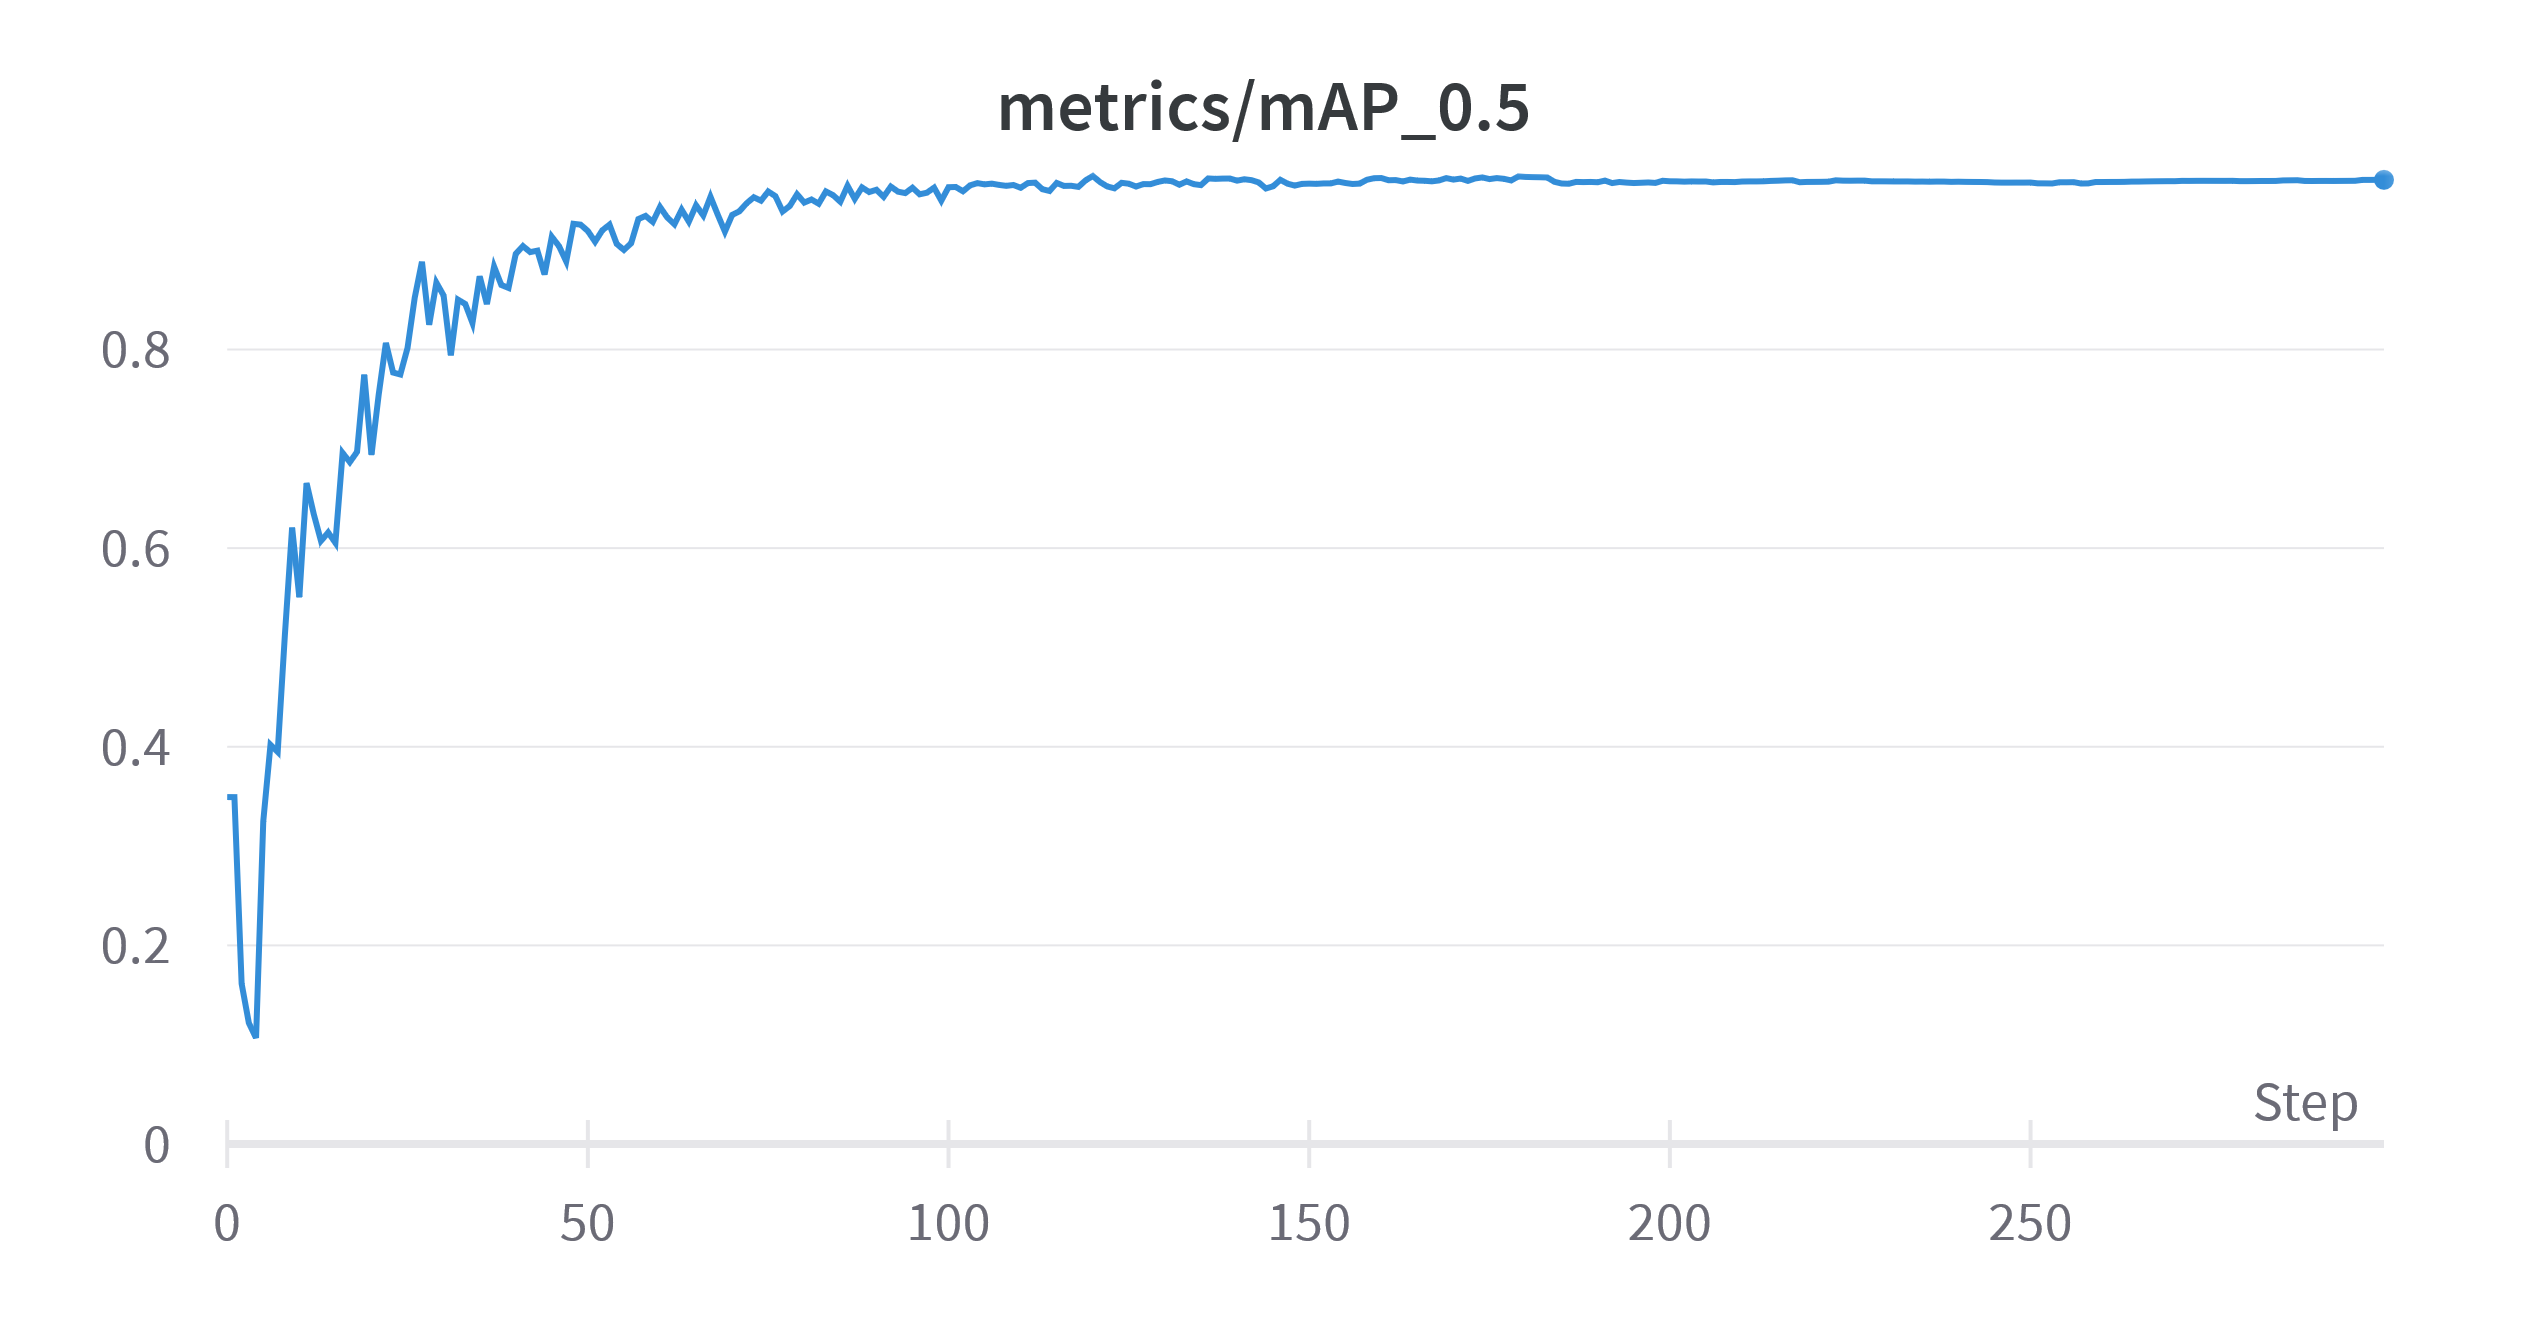
\includegraphics[scale=0.07]{metricsmAP_0.5.png}}}
	\subfloat[mAP@.5:.95]{{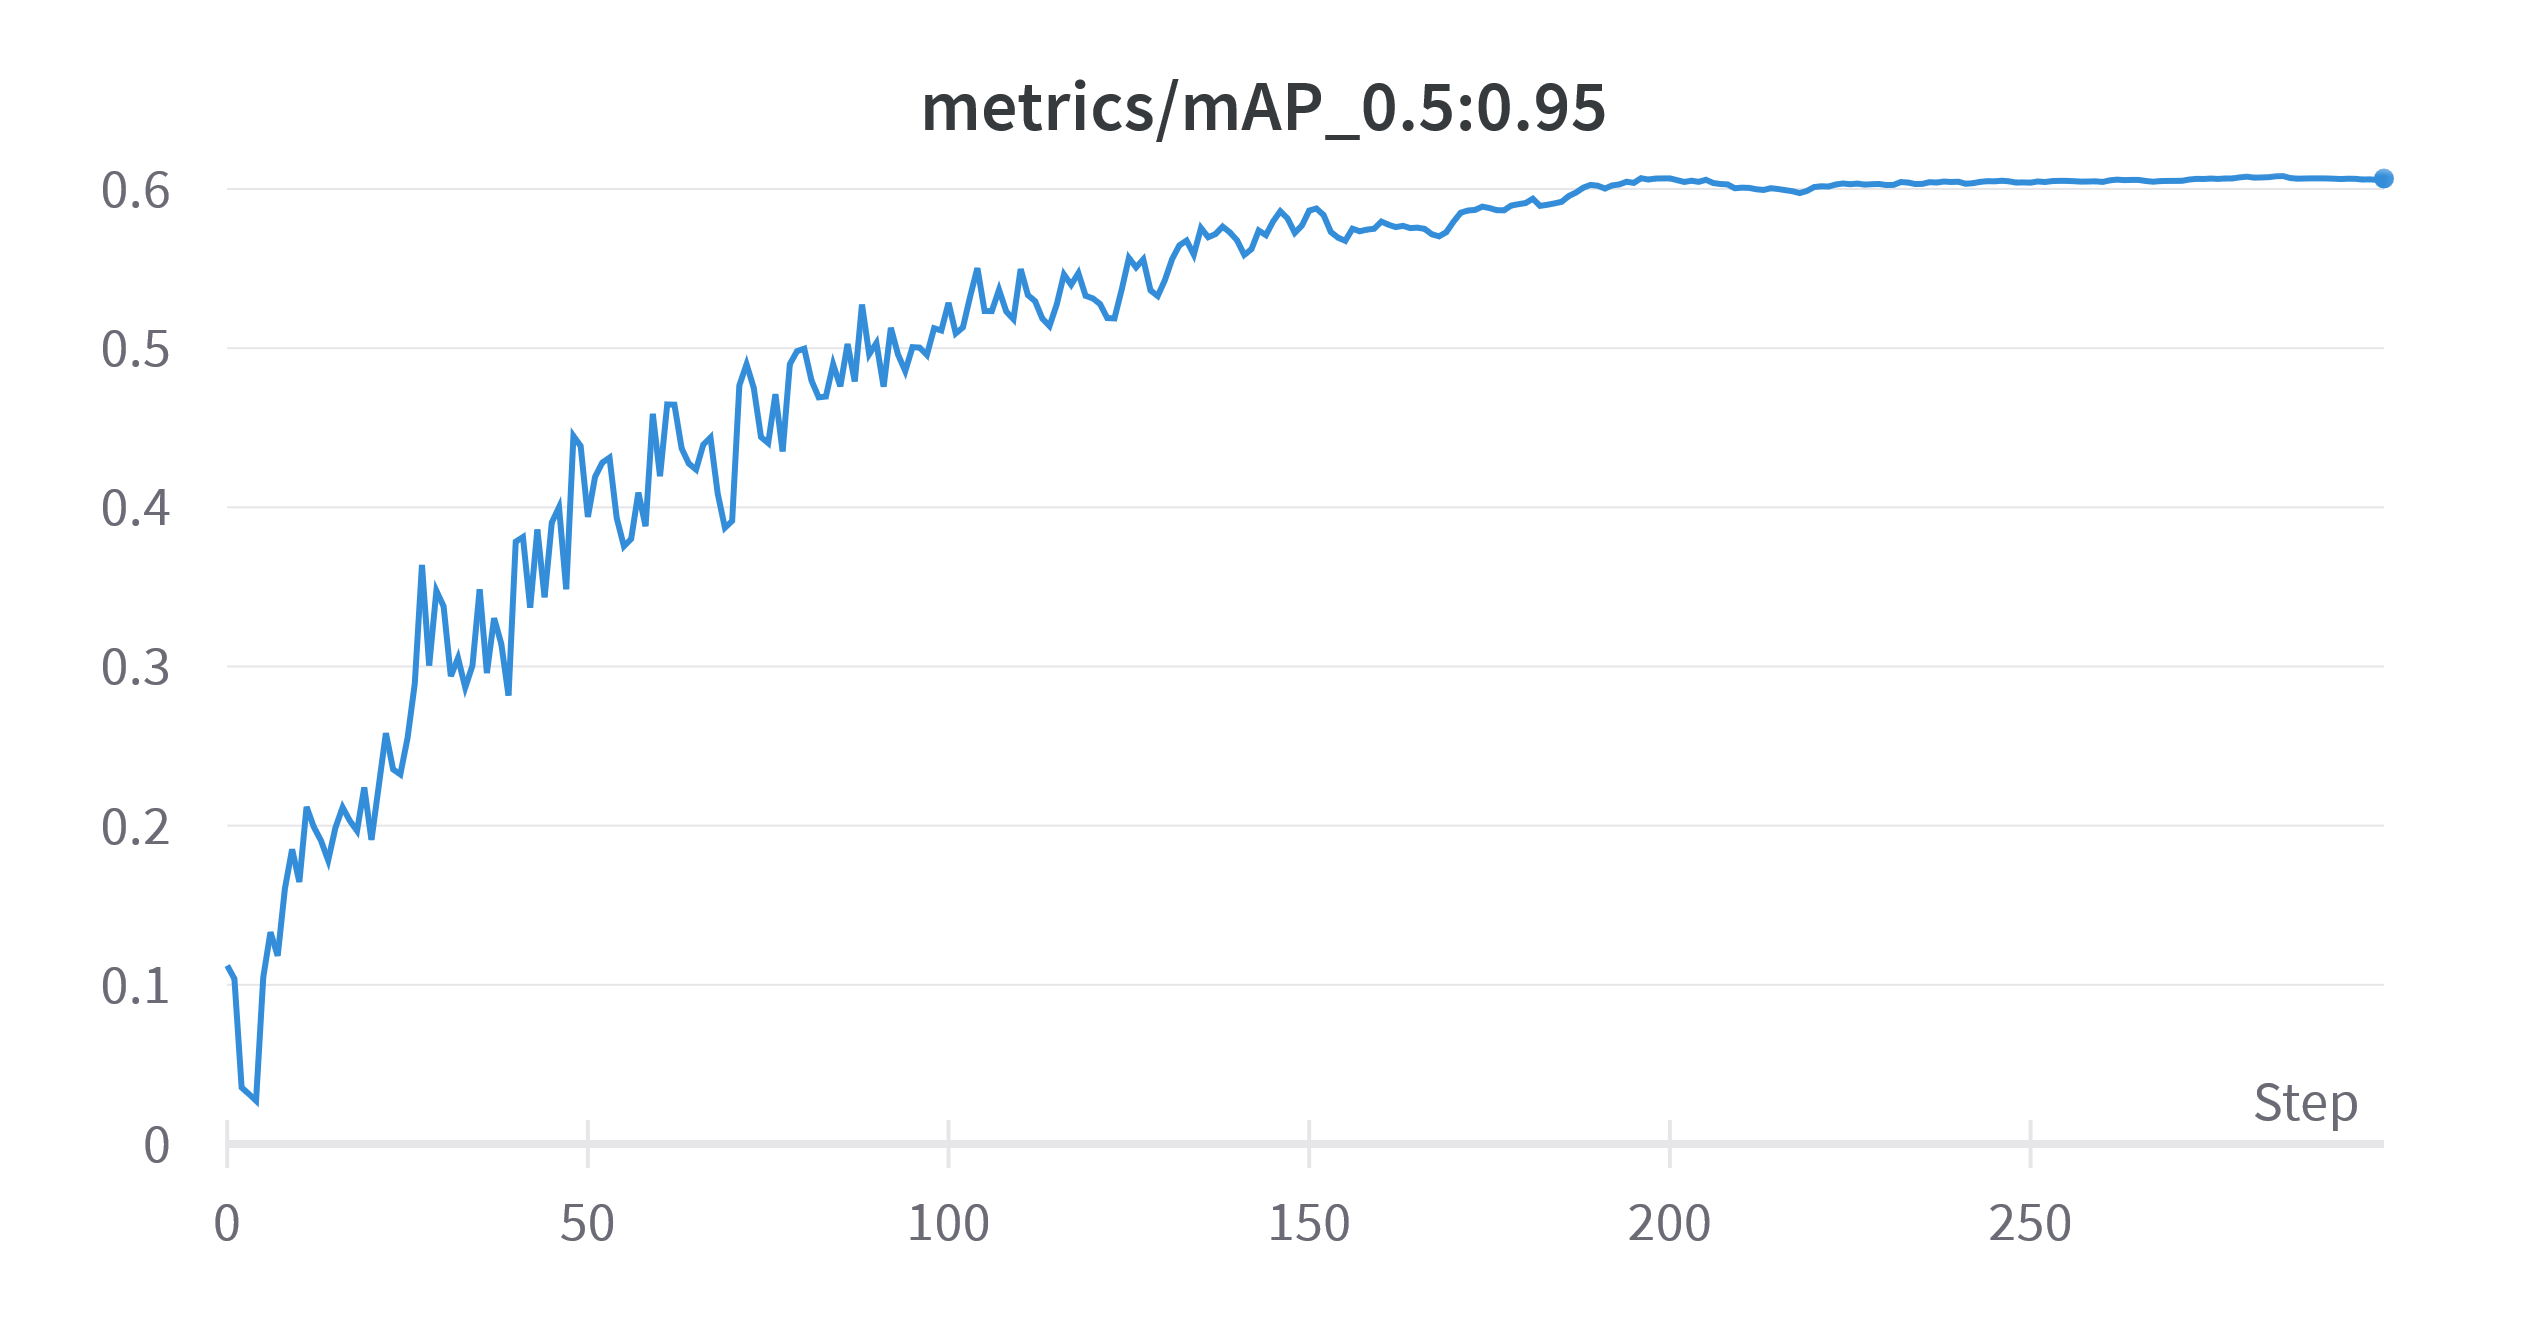
\includegraphics[scale=0.07]{metricsmAP_0.5_0.95.png}}}
\caption{Performances de notre modèle après entrainement.}
\label{fig:ai_results}
\end{figure}
\FloatBarrier

Les différentes définitions peuvent être retrouvées en annexe (\ref{appendix:mAP}).\\
%Nombre de vrai positif divisé par le nombre de vrai positif plus le nombre de faux positif
%Nombre de vrai positif divisé par le nombre de positif total
\\
Les résultats obtenus sont compilés dans le tableau suivant:\\
\begin{center}
\begin{tabular}{|c|c|c|c|}
	\hline
	Précision & Recall & mAP@.5 & mAP@.5:.95\\
	\hline
	0.953 & 0.959 & 0.971 & 0.607\\
	\hline
\end{tabular}
\end{center}

\begin{figure}[!htbp]
\center
	\subfloat{{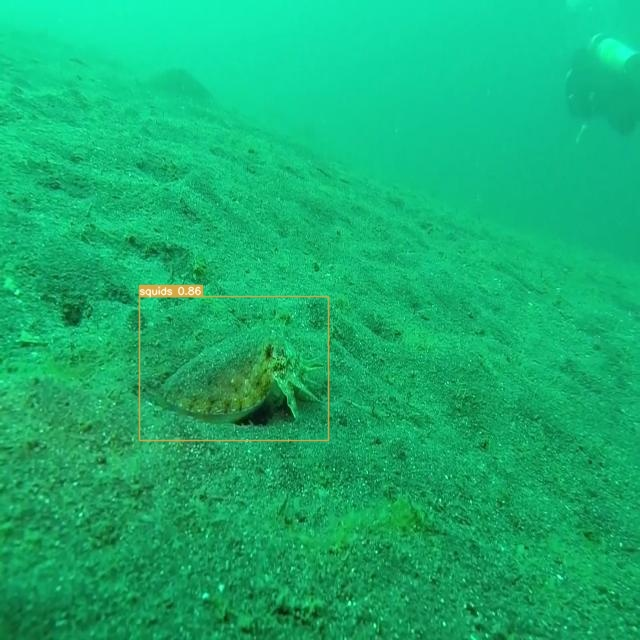
\includegraphics[scale=0.3]{cuttlefish_example1.jpg}}}
	\hspace{0.1cm}
	\subfloat{{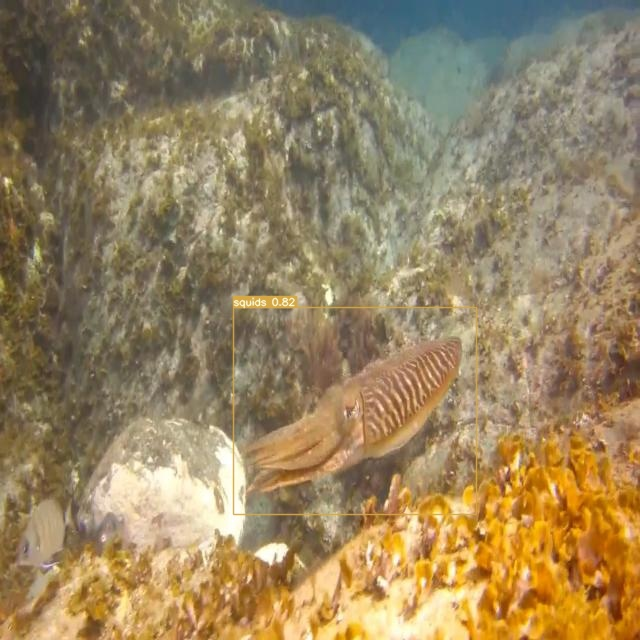
\includegraphics[scale=0.3]{cuttlefish_example2.jpg}}}
	\\
	\subfloat{{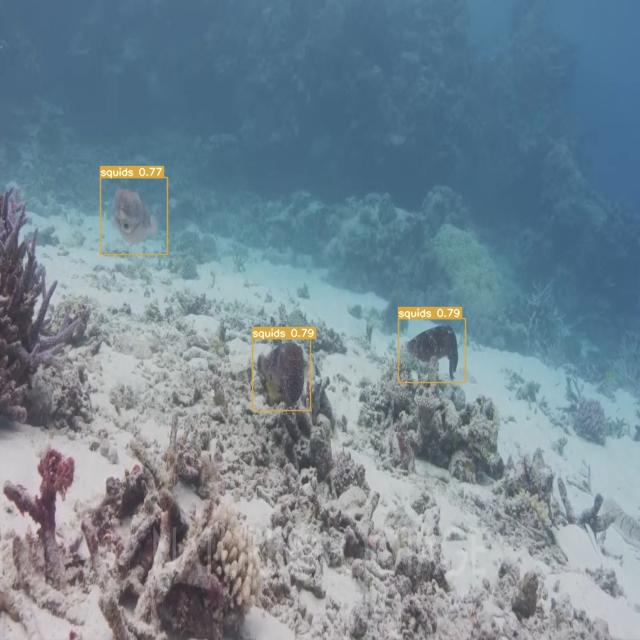
\includegraphics[scale=0.3]{cuttlefish_example3.jpg}}}
	\hspace{0.1cm}
	\subfloat{{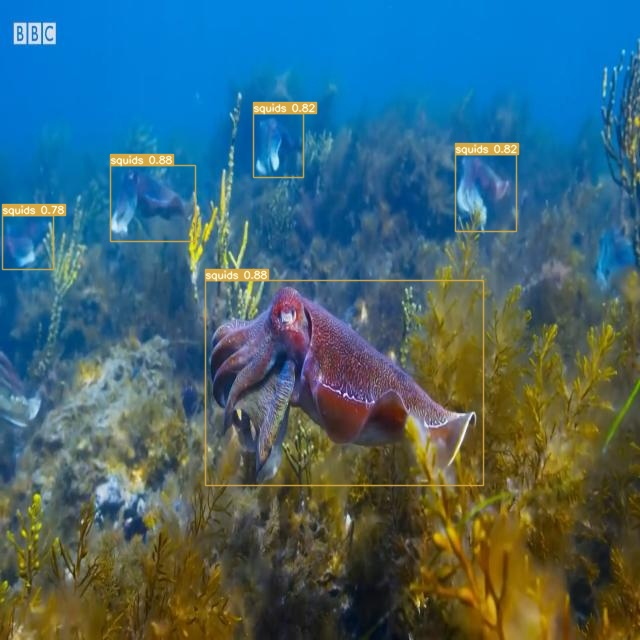
\includegraphics[scale=0.3]{cuttlefish_example4.jpg}}}
\caption{Exemples de résultats obtenus par notre modèle.}
\label{fig:ai_examples}
\end{figure}
\FloatBarrier



\section{Modules}

\subsection{Descripteurs}
\subsection{Mesure de similarité}
\subsection{Filtre à particule}

\begin{figure}[!htbp]
\center
	\subfloat{{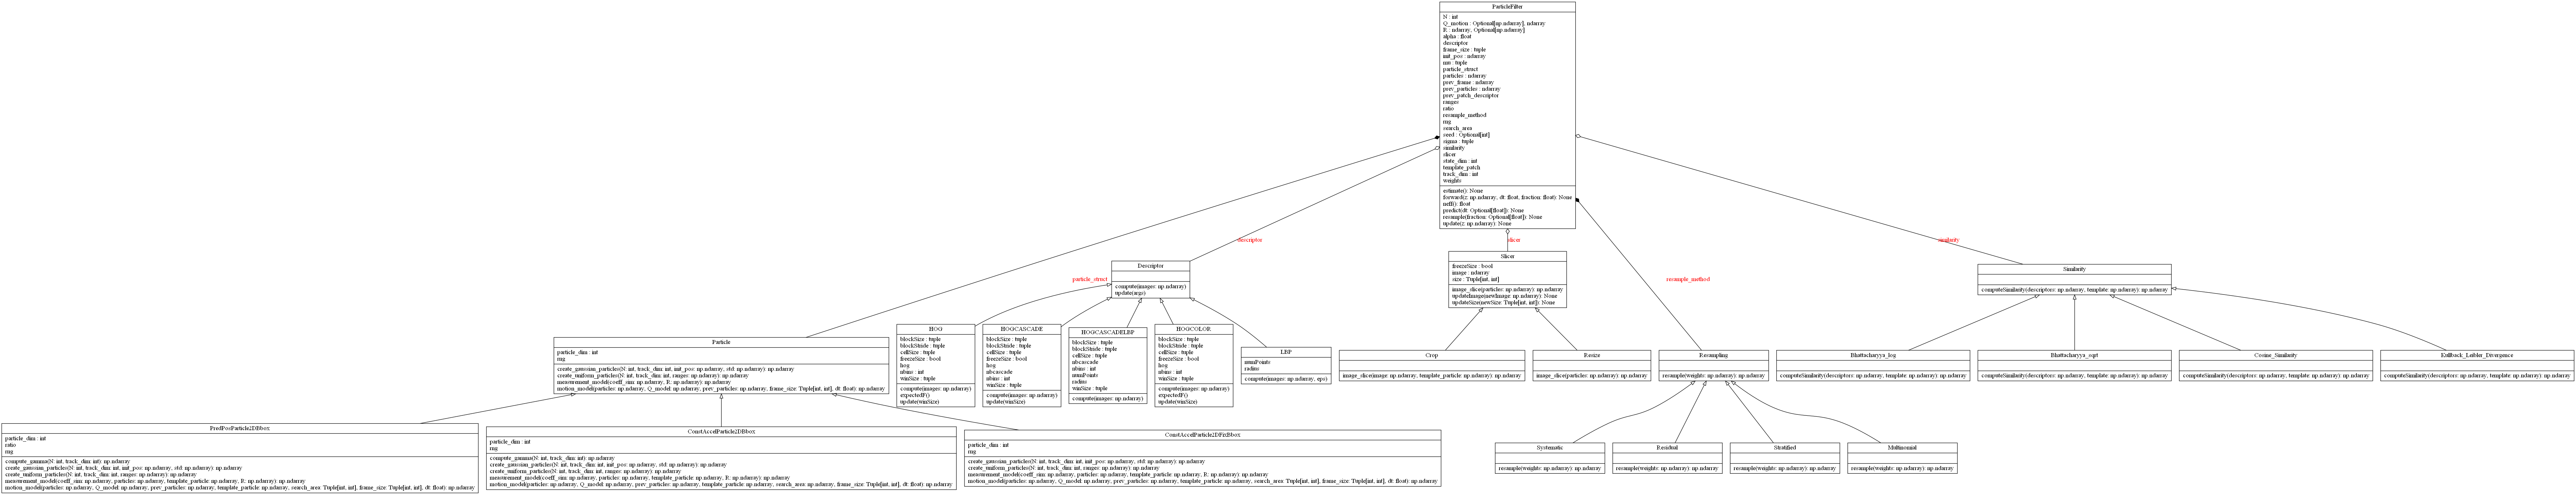
\includegraphics[scale=0.065]{particlefilter.png}}}
\caption{Diagramme UML des classes du module filtre à particule.}
\label{fig:uml_diagram_particlefilter}
\end{figure}
\FloatBarrier

\begin{figure}[!htbp]
\center
	\subfloat{{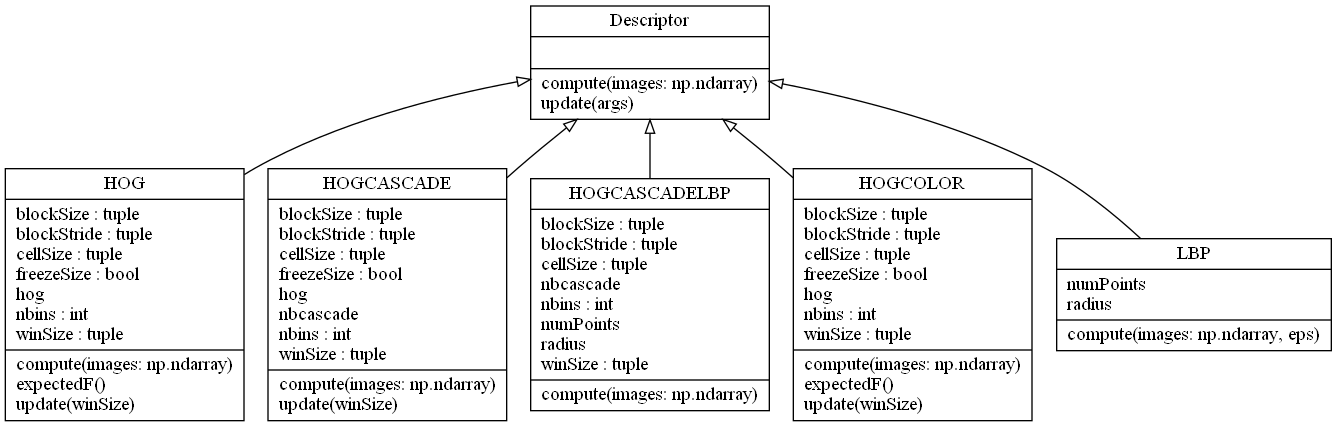
\includegraphics[scale=0.4]{descriptors.png}}}
\caption{Diagramme UML des classes du module descripteur.}
\label{fig:uml_diagram_classes}
\end{figure}
\FloatBarrier

\begin{figure}[!htbp]
\center
	\subfloat{{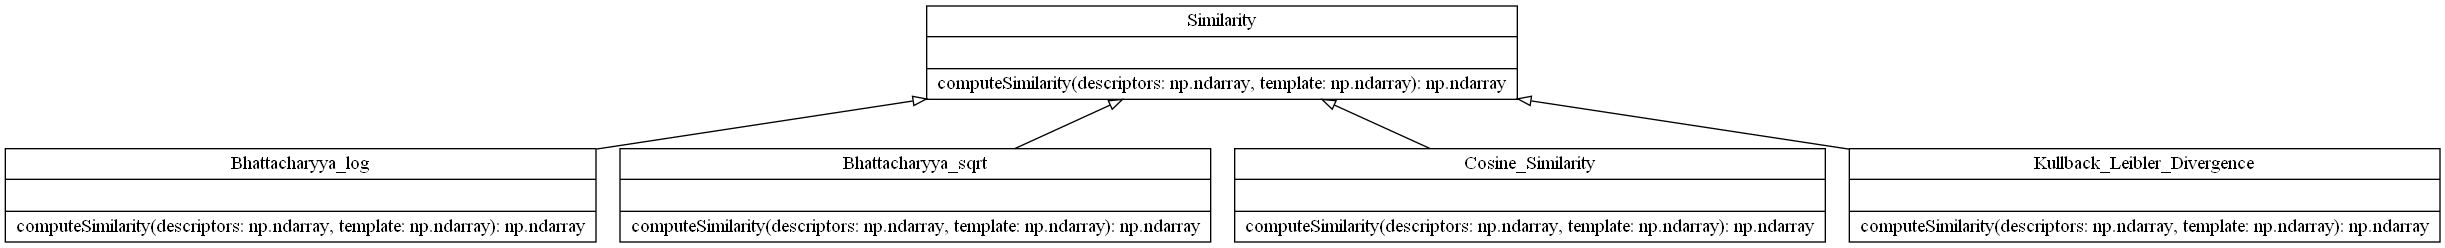
\includegraphics[scale=0.2]{similarity.png}}}
\caption{Diagramme UML des classes du module mesure de similarité.}
\label{fig:uml_diagram_classes}
\end{figure}
\FloatBarrier

\begin{figure}[!htbp]
\center
	\subfloat{{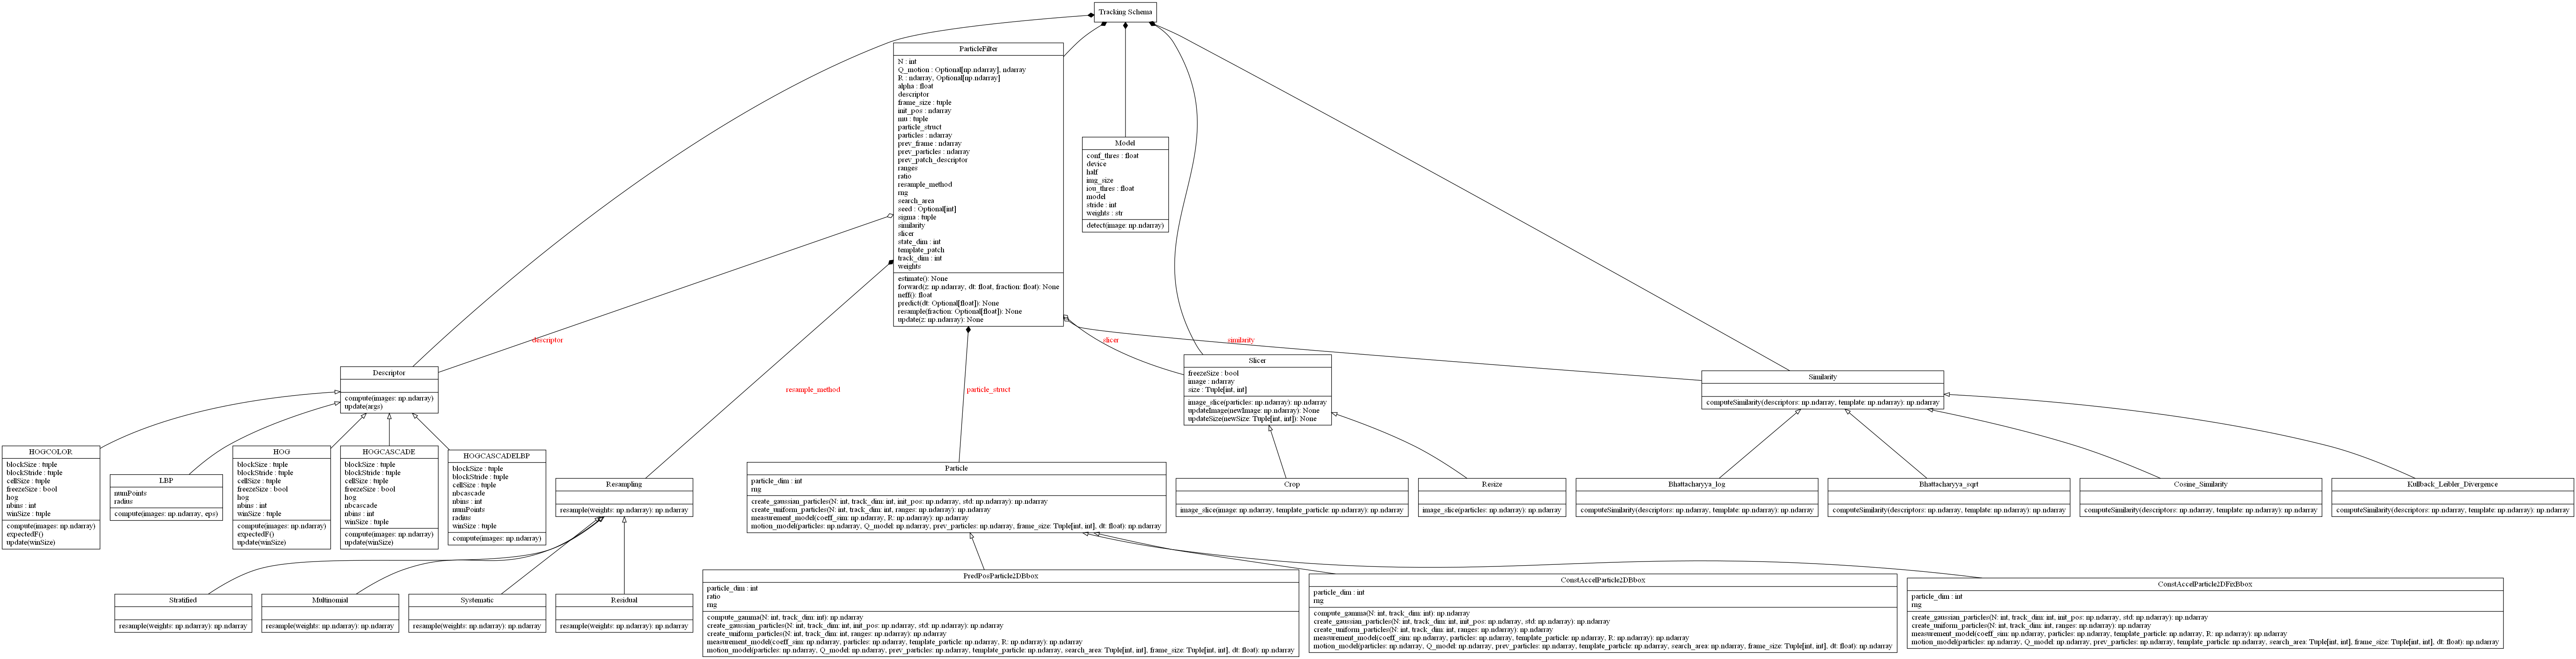
\includegraphics[scale=0.085]{classes.png}}}
\caption{Diagramme UML des classes global.}
\label{fig:uml_diagram_classes}
\end{figure}
\FloatBarrier

\begin{figure}[!htbp]
\center
	\subfloat{{
\includegraphics[scale=0.4]{usecase.png}}}
\caption{Diagramme UML de cas d'utilisation.}
\label{fig:uml_diagram_usecase}
\end{figure}
\FloatBarrier




\section{Structures de données}
Les structures de données principales du projet sont les tenseurs en tant que tableau multidimensionnel, pour ce faire, nous utilisons la librairie Numpy, qui permet de réaliser des opérations sur ces tableaux de façon optimisé.\\
Nous essayons de garder les données un maximum sous ce format, pour éviter les conversions et opérations qui pourraient ralentir le logiciel de suivi. C'est pour cela que la majorité des entrées des programmes réalisés demande des 'ndarray', qui est le type des tableaux Numpy.\\
\\
Les images prisent en entrée des programmes sont transformées en tableau Numpy, selon la convention de OpenCV, c'est-à-dire avec les couleurs au format BGR et la hauteur de l'image comme première dimension du tenseur, et la largeur de l'image comme seconde dimension.\\
\\
L'utilisateur du logiciel n'intervient qu'à un seul niveau dans le programme, le reste des entrées du logiciel est géré en interne afin de préserver au mieux l'intégrité des données traitées.\\
L'utilisateur peut uniquement donner des paramètres au logiciel lorsqu'il le lance, ces paramètres sont alors parser en différent arguments qui sont vérifiés par le programme, puis utilisés pour initialiser les différents module, afin de commencer le suivi d'une seiche.




\section{Statistiques}
Le projet compte un total de 25 classes réparties dans 10 scripts python (voir figure \ref{fig:uml_diagram_classes}).\\
Les scripts et classes de YOLOv7\cite{wang_yolov7_nodate} utilisés dans le projet ne sont pas comptés.\\
Le projet compte en tout 1576 lignes de code.\\
L'entièreté du projet est en accès libre sur github (\cite{pp2pf}).

\clearpage